\documentclass[11pt,a4paper]{article}

% ---------------------------------------------------------------------------
% Packages. The build machine's TeX Live lacks tikz/pgf, lmodern, cm-super,
% enumitem, xurl and multirow, so the paper uses Computer Modern in OT1, plain
% list environments and a matplotlib-drawn vector figure (figures/architecture.py).
% ---------------------------------------------------------------------------
\usepackage[utf8]{inputenc}
\usepackage[margin=2.5cm]{geometry}
\usepackage{amsmath}
\usepackage{graphicx}
\usepackage{booktabs}
\usepackage{tabularx}
\usepackage{array}
\usepackage[table]{xcolor}
\usepackage[expansion=false]{microtype} % font expansion needs scalable fonts for every face used
\usepackage{caption}
\usepackage[numbers,sort&compress]{natbib}
\usepackage{url}
\usepackage[colorlinks=true,linkcolor=blue!50!black,citecolor=blue!50!black,urlcolor=blue!50!black]{hyperref}

% Allow long URLs and identifiers to break anywhere sensible.
\makeatletter
\g@addto@macro{\UrlBreaks}{\do\a\do\b\do\c\do\d\do\e\do\f\do\g\do\h\do\i\do\j\do\k\do\l\do\m
  \do\n\do\o\do\p\do\q\do\r\do\s\do\t\do\u\do\v\do\w\do\x\do\y\do\z\do\_\do\-\do\.\do\/}
\makeatother

% Configuration keys and wire identifiers, e.g. \cfg{front.total_budget_ms}.
\DeclareUrlCommand\cfg{\urlstyle{tt}}

% Placeholder for numbers measured in the evaluation (written separately).
\newcommand{\result}[1]{\textbf{[RESULT: #1]}}

\setlength{\parskip}{0.35em}
\renewcommand{\labelitemi}{$\bullet$} % avoids a bitmap TS1 bullet (cm-super is not installed)
\renewcommand{\arraystretch}{1.12}

\title{\textbf{Bud WaaV Interaction Mode:\\an Open, Self-Hosted Runtime for Voice Agents\\That Keep Talking While They Work}}
\author{Bud Ecosystem\\[0.3em]
  \normalsize Bud Ecosystem Inc.\\
  \normalsize \texttt{waav@bud.studio}\\
  \normalsize \url{https://github.com/BudEcosystem/WaaV}}
\date{27 October 2026 \quad (WaaV Gateway release 1.1.0)}

\begin{document}
\maketitle

\begin{abstract}
\noindent
A voice agent that works with tools is caught between two failures: a turn-based pipeline goes silent while
its model and tools run, and a fast end-to-end speech model tends to take the floor when the caller has only
paused. Recent systems split the agent into a fast interaction model that stays in the conversation and a
slower background model that does the work; the published ones are closed and hosted. We describe
\emph{interaction mode} of Bud WaaV, an open-source (Apache-2.0), self-hosted implementation of this split in a
real-time voice gateway. A 2B-parameter front model (Qwen3.5-2B on llama.cpp) decides every caller turn into
one explicit, grammar-constrained act (a request, a correction, a cancellation, a conversation control, a status
question or a wait) and acknowledges at once. Requests become tasks that run on any language model, on an
orchestrator that hands work to agents as child tasks, or on agents reached over A2A, MCP, webhooks or the
OpenAI Responses API; answers are relayed verbatim, sentence by sentence, and side-effecting actions wait for a
confirmation the caller has heard. The audio path tracks the floor, ducks the agent at the caller's onset,
classifies overlap within 900\,ms and gates echo, and every slot can be filled by one of 44 speech vendors or a
local model. On Full-Duplex-Bench v3, which plays 100 real, disfluent spoken requests to an agent with tools,
Bud WaaV with Claude Opus~5.5 as its background starts speaking sooner than every published system (2.48\,s
mean against 3.88--8.78\,s) with the second-best response quality (0.73), but its strict task success is the
lowest (Pass@1 0.39 judged, 0.31 exact-match, against 0.41--0.60), as is its tool-selection F1; most of the
failures trace to the turn handling around the background model (a disfluent pause that ends the turn, one
request split into several tasks), which we analyse. On
Full-Duplex-Bench v1 it keeps quiet through the caller's pauses as well as the best closed systems (it takes
the floor in 2.9\% of synthetic and 9.7\% of real pauses, the latter the lowest on the leaderboard) and makes
listening sounds more often than any system on it, at the cost of fewer and slower turn takings (78\%, 1.28\,s) and slow replies to interruptions (2.21\,s). A case study shows a spoken conversation in which the caller hands a browser, a terminal and a word
processor real work one request at a time, chatting in between, each request acknowledged within 1.8\,s and
the one action that changes something confirmed by a heard yes; the takes behind it found gateway defects that
we fixed and report.
A cascade keeps a latency floor that end-to-end models avoid; we discuss what the
explicit decision, the task layer and the confirmations buy in exchange.
\end{abstract}

\noindent\textbf{Keywords:} full-duplex spoken dialogue; voice agents; turn-taking; barge-in;
asynchronous tool use; background tasks; human in the loop; open source.

\section{Introduction}\label{sec:intro}

People take turns quickly. In recordings of ten languages, answers to yes/no questions most often began
within about 200\,ms of the end of the question~\citep{stivers2009universals}, which implies that
listeners plan their response while the other person is still talking~\citep{levinson2015timing}.
Listeners also signal attention while the other person talks, give way when interrupted, and do not
treat every pause as an invitation to speak~\citep{sacks1974turntaking,skantze2021review}. A voice agent
that must \emph{do} something on a call, such as look up an order or change a booking, faces a harder
version of this problem: the work may take seconds or minutes, the caller keeps talking while it runs,
and some of what the caller says changes the work (``actually, make it eight'').

A classical cascade of speech-to-text, a language model and text-to-speech answers only after the whole
chain has run. On Full-Duplex-Bench v3, a benchmark of tool use under real disfluency, a
Whisper$\to$GPT-4o$\to$TTS cascade spoke its first words 8.78\,s after the end of the user's speech, later
than any other system tested, and completed the task after 10.12\,s~\citep{lin2026fdbv3}. End-to-end full-duplex models remove most of that delay but
trade it for floor control: on the Full-Duplex-Bench v1 leaderboard Moshi starts its response 0.265\,s
after the user stops but takes the floor in 98.5\% of synthetic pauses, while the GPT-Realtime entry does
so in 1.0\% of them and responds after 1.470\,s~\citep{fdb_repo,lin2025fdbv1}. Neither end of this
trade-off suits an agent that must also act.

In 2026 a third design became prominent. Thinking Machines Lab's \emph{interaction models} pair a
real-time interaction model, which processes audio in 200\,ms micro-turns, with an asynchronous background
model for reasoning and tool use that shares its context; the interaction model is a 276B-parameter
mixture-of-experts (12B active) trained from scratch, and the system was announced as a research
preview~\citep{tml2026interaction}. OpenAI's GPT-Live
delegates search and reasoning to a backend model behind an asynchronous
boundary~\citep{openai2026gptlive,openai2026gptlivesys}, Google's Gemini 3.8 Live runs tools in the
background while it keeps talking~\citep{google2026g38}, and open frameworks have added asynchronous tool
calls~\citep{livekit2026async,pipecat_fc}. The front/background split is therefore not new. What is
missing is an implementation that an operator can run on its own hardware, with its own choice of speech
vendors, models and agents, and inspect.

This paper describes \emph{interaction mode}, released in Bud WaaV Gateway 1.1.0 on 27 October
2026~\citep{waav_repo,waav_imdoc}. WaaV is an open-source (Apache-2.0) real-time voice gateway written in
Rust. Interaction mode adds a small \emph{front model} (Qwen3.5-2B~\citep{qwen35_2b} on
llama.cpp~\citep{llamacpp}) that names one explicit \emph{act} for every caller turn and acknowledges at
once; a \emph{task layer} that runs each request on any language model, an orchestrator or remote agents
and relays the answer verbatim; a \emph{duplex audio layer} that tracks the floor, yields to the caller and
ignores its own echo; and a \emph{policy layer} that guarantees that the words that bind (confirmations and
reports of what was done) come from templates and from the background's own text, never from the small
model. Our contributions are:
\begin{itemize}
  \item an open, self-hostable design in which a 2B front model makes an explicit, grammar-constrained,
    logged decision per caller turn while the gateway owns the binding words
    (Sections~\ref{sec:sys-front}--\ref{sec:sys-policy});
  \item background work as first-class tasks with revisions, committed-effect accounting, speculative
    start, an update inbox, follow-ups and life after the call, behind one open task protocol over
    webhooks, A2A, MCP and the OpenAI Responses API (Sections~\ref{sec:sys-tasks}--\ref{sec:sys-backgrounds});
  \item duplex behaviour inside a cascade, with a timeline of what the caller heard that decides when a
    spoken answer binds, and confirmations by voice, screen or keypad (Sections~\ref{sec:sys-audio}
    and~\ref{sec:sys-hitl});
  \item the same mode over 44 speech vendors, 11 speech-to-speech integrations, LiveKit rooms and SIP calls
    (Section~\ref{sec:sys-surfaces}), with measurements on Full-Duplex-Bench v1 and v3
    (Section~\ref{sec:eval}) and a case study (Section~\ref{sec:case}).
\end{itemize}
We do not claim that the design beats end-to-end models on every axis. A cascade has a latency floor
(the time to settle the end of a turn plus the time to the first synthesised audio) that a single model
trained on audio does not have. WaaV addresses \emph{perceived} latency, by acknowledging at once and
keeping the caller informed while work runs, and makes the agent's decisions explicit;
Section~\ref{sec:discussion} discusses the trade-off and the known limits of the release.

\section{Related Work}\label{sec:related}

Numbers in this section are taken from the cited sources; numbers that vendors or authors report about
their own systems are marked \emph{self-reported} (SR). Latency metrics differ between sources and are
comparable only when the metric is the same.

\paragraph{Turn-taking.}
Conversation analysis describes turn-taking as locally managed, with speaker changes at
transition-relevance places~\citep{sacks1974turntaking}; \citet{skantze2021review} reviews how spoken
dialogue systems detect turn ends and handle backchannels and interruptions, and Voice Activity
Projection learns to predict both speakers' future activity from audio~\citep{ekstedt2022vap}. Practical
agents pair a voice activity detector with an end-of-turn classifier on the audio, such as Smart Turn, an
8M-parameter model on a Whisper-Tiny encoder~\citep{smartturn_repo,daily2025smartturnv3}, or on the
transcript, such as LiveKit's text turn detector~\citep{livekit_turndetector}. Sesame's TurnBench evaluates
such detectors and concludes that ``no system is fast, selective, and high-recall at the same
time''~\citep{sesame2026turnbench}.

\paragraph{End-to-end full-duplex models.}
dGSLM~\citep{nguyen2023dgslm}, Moshi~\citep{defossez2024moshi}, Freeze-Omni~\citep{wang2024freezeomni} and
PersonaPlex~\citep{roy2026personaplex} model both sides of a conversation directly from audio; NemotronLabs VoiceChat
adds tool calls but states that ``users cannot interrupt during tool execution''~\citep{nvidia2026voicechat}. None of
the open models runs background work while it talks, and on Full-Duplex-Bench v1 their low turn latency often comes
with a high rate of taking the floor during the user's pauses~\citep{fdb_repo}.

\paragraph{Interaction models with a background model.}
A fast responder backed by a slow deliberator echoes dual-process accounts of thinking~\citep{kahneman2011thinking}
and talker--reasoner agent architectures~\citep{christakopoulou2024talker}. TML's interaction model works in
200\,ms chunks beside an asynchronous background model with shared context and reports a Full-Duplex-Bench v1
turn-taking latency of 0.40\,s and, with the background agent, a v3 Pass@1 of 68.0\% (SR)~\citep{tml2026interaction}.
GPT-Live is a full-duplex voice layer that delegates to a backend text model, possibly a third-party one, priced at
USD 0.05 per minute for the voice layer alone~\citep{openai2026gptliveapi}. Gemini 3.8 Live makes non-blocking
function calls the default, with results delivered silently, when idle or by interrupting~\citep{google_livecap},
and gpt-realtime supports asynchronous function calls, MCP and SIP~\citep{openai2025gptrealtime}. All are closed and
hosted, use the vendor's own voices and recognisers, and do not expose the per-turn decision they make.

\paragraph{Cascade frameworks and hosted platforms.}
Pipecat (BSD-2-Clause) composes services from many vendors, with 38 speech-to-text, 59 text-to-speech, 32 language-model
and 11 speech-to-speech services listed~\citep{pipecat_services}; its asynchronous functions keep the conversation
going while they run, and it documents no caller-confirmation pattern~\citep{pipecat_fc}. LiveKit Agents (Apache-2.0)
added asynchronous tools in June 2026, with immediate acknowledgement, progress and cancellation and an option that
re-asks before a \emph{duplicate} call~\citep{livekit2026async}; its adaptive interruption model is
cloud-only~\citep{livekit2026adaptive}. Kyutai's Unmute is an open cascade without a task layer~\citep{kyutai_unmute}.
The documentation of Vapi, Retell, Deepgram's Voice Agent and ElevenLabs Agents describes neither talking while a tool
runs (beyond an undocumented ``Async'' toggle in Vapi) nor a confirmation gate~\citep{vapi_tools,retell_interrupt,deepgram_fc,elevenlabs_toolint}.
Table~\ref{tab:related} summarises the comparison.

\begin{table}[t]
\centering
\caption{Systems for interactive voice agents as documented on 27 October 2026. ``Background'': the agent keeps
talking while tools or agents run. ``Confirm'': a documented gate that asks the caller before a side-effecting
action. Latencies use different metrics and are not comparable across rows; SR = self-reported.}
\label{tab:related}
\footnotesize
\begin{tabularx}{\textwidth}{@{}>{\raggedright\arraybackslash}p{2.6cm}>{\raggedright\arraybackslash}X>{\raggedright\arraybackslash}p{1.15cm}>{\raggedright\arraybackslash}p{1.75cm}>{\raggedright\arraybackslash}p{1.55cm}>{\raggedright\arraybackslash}p{2.75cm}@{}}
\toprule
System & Architecture & Open, self-host & Background & Confirm & Reported latency \\
\midrule
TML interaction models~\citep{tml2026interaction} & 276B MoE interaction model, 200\,ms micro-turns, background model & no & yes & not documented & FDB v1 turn 0.40\,s (SR) \\
GPT-Live-1~\citep{openai2026gptliveapi} & voice layer + backend text model & no & yes & not documented & none published \\
gpt-realtime~\citep{openai2025gptrealtime} & speech-to-speech model & no & async calls & not documented & FDB v1 turn 1.470\,s~\citep{fdb_repo} \\
Gemini Live 3.8; 3.1 Flash~\citep{google2026g38,google_g31doc} & native audio & no & 3.8: yes; 3.1: no & not documented & 3.1 (minimal): FDB v1 turn 0.567\,s~\citep{fdb_repo} \\
Moshi; PersonaPlex~\citep{defossez2024moshi,roy2026personaplex} & full-duplex, 7B backbone & yes & no tools & n/a & FDB v1 turn 0.265\,s; 0.070\,s (SR; 0.170\,s released) \\
NemotronLabs VoiceChat~\citep{nvidia2026voicechat} & 11B full-duplex & research only & no interrupt during tools & not documented & FDB v1 turn 448\,ms (SR) \\
Kyutai Unmute~\citep{kyutai_unmute} & open cascade & yes & no & no & ``below a second'' (SR) \\
Pipecat; LiveKit Agents~\citep{pipecat_fc,livekit2026async} & cascade frameworks & yes; partly & async tools & duplicates only (LiveKit) & not reported \\
Vapi, Retell, Deepgram, ElevenLabs~\citep{vapi_tools,retell_interrupt,deepgram_fc,elevenlabs_toolint} & hosted cascades & no & not documented & no & vendor claims \\
\midrule
Bud WaaV interaction mode & cascade + 2B front model; tasks on any LLM or agent & yes & yes, as tasks & voice, screen, keypad & FDB v1 turn 1.28\,s; pause TOR 0.029 (Sec.~\ref{sec:eval-v1}) \\
\bottomrule
\end{tabularx}
\end{table}

\paragraph{Benchmarks.}
Full-Duplex-Bench v1 scores pause handling, backchanneling, smooth turn-taking and user interruption with takeover rates
(TOR) and latencies~\citep{lin2025fdbv1}; v1.5 adds overlap scenarios without defining an aggregate score, so TML's
``v1.5 average'' is its own composite~\citep{lin2025fdbv15}; v2 runs multi-turn sessions with an automated
examiner~\citep{lin2026fdbv2}; and v3 evaluates tool use on 100 real recordings with disfluencies~\citep{lin2026fdbv3}.
FLEXI adds model-initiated interruptions~\citep{ge2025flexi}, while VoiceBench~\citep{chen2024voicebench}, Big Bench
Audio~\citep{aa_bigbenchaudio} and Audio MultiChallenge~\citep{gosai2025audiomc} measure understanding rather than
turn-taking; Talk Arena found that no static benchmark correlated strongly with interactive preference~\citep{li2025mindthegap}.

\section{System}\label{sec:system}

This section describes interaction mode as released in WaaV Gateway 1.1.0. The reference
documentation~\citep{waav_imdoc} specifies every setting, event and message, and the design chapters and
contracts~\citep{waav_design} record why each mechanism exists; where they differ, we describe the released
behaviour. Configuration keys are set in \texttt{typewriter} type; all values quoted are
configured defaults, not measurements.

\begin{figure}[t]
\centering
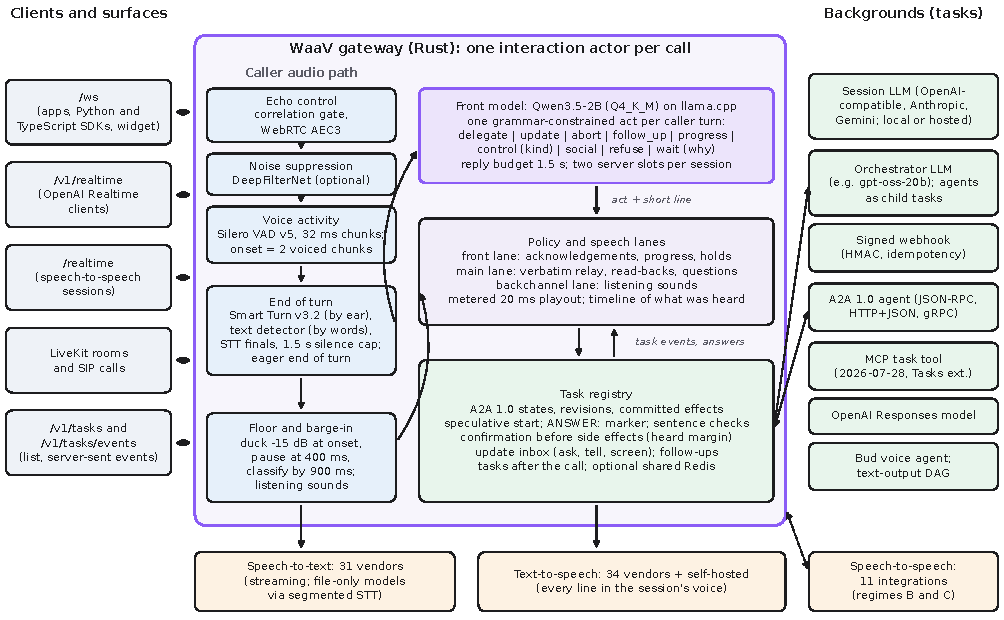
\includegraphics[width=\textwidth]{figures/architecture.pdf}
\caption{Architecture of interaction mode. Clients reach the gateway over several surfaces (left). Each call has
one interaction actor: the caller's audio passes echo control, optional noise suppression, voice activity and
end-of-turn detection, which feed the floor and barge-in machine and, with the transcripts, the front model. The
front model names one act per caller turn; the policy engine schedules speech on three lanes; the task registry
runs requests on background models and agents (right) and relays their answers. Speech-to-text and text-to-speech
(bottom) come from any supported vendor or a self-hosted model; a speech-to-speech provider can replace the
cascade's voice.}
\label{fig:arch}
\end{figure}

\subsection{Overview}\label{sec:sys-overview}

WaaV sits between a client application and speech providers: the client streams audio or text to one endpoint,
and the gateway transcribes it, runs the agent and streams the synthesised reply back, with the providers the
session names~\citep{waav_repo}. Interaction mode is opt-in. A session runs it when the server switch
(\cfg{interaction.enabled}) is on, the session or the operator asks for it, a background exists to run requests,
the speech-to-text provider can end an utterance and keep listening, and a language pack covers the session's
language; otherwise the session receives one \cfg{config_warning} and behaves as without the mode.

Each session has one \emph{interaction actor} that owns the call's state and handles its inbox one message at a
time, running deterministic state machines (duplex engine, floor, policy, lane executor) and spawning every effect
that needs I/O, so timing rules can be tested on a virtual clock~\citep{waav_design}. The design separates three
roles (Figure~\ref{fig:arch}). The \emph{front} decides what each caller turn is and says short lines at once. The
\emph{background} does the requested work as a \emph{task}. The \emph{gateway} owns timing and the words that bind:
it relays the background's answers word for word and words every confirmation, question and failure notice from
templates. The front's prompt forbids it to say a number, date, name or availability the caller did not say, to
predict an outcome, or to say that something is done.

\subsection{Turn-taking, floor and duplex audio}\label{sec:sys-audio}

\paragraph{End of turn.}
Every caller frame is copied, without delaying speech-to-text, into a per-session analyser that runs Silero VAD
v5~\citep{silero_vad} on 32\,ms chunks and confirms the caller's onset after two voiced chunks (64\,ms). A turn ends
when the recogniser ends its segment, earlier when Smart Turn v3.2~\citep{smartturn_repo}, asked 200\,ms into each
pause, is sure the caller has finished, and at the latest after 1.5\,s of silence; release builds also run the
LiveKit text turn detector~\citep{livekit_turndetector} on final transcripts. A thinking pause is \emph{held}: a final
transcript does not end the turn when Smart Turn is unsure (below 0.7) and the words end on one that leaves the
sentence open (``and'', ``to''), and a held turn ends 800\,ms later unless the caller goes on. Turns begun over the
agent and answers to the agent's questions are never held. With \cfg{duplex.eager} the gateway also acts on a likely
end of turn before the final transcript by starting a provisional background run (Section~\ref{sec:sys-tasks}).

\paragraph{Floor and heard audio.}
The gateway reports who holds the floor (\texttt{user}, \texttt{assistant}, \texttt{both} or \texttt{none}). The
agent's audio leaves through a metered pump that paces 20\,ms frames on a playout clock and holds everything beyond
a short lead (150\,ms on a WebSocket, 40\,ms in a LiveKit room), so a duck or a cut acts on audio not yet heard.
From delivered frames and the client's playback reports the gateway keeps a timeline of what the caller heard; it
decides when a spoken ``yes'' binds (Section~\ref{sec:sys-hitl}), what ``say that again'' repeats, and what the
background is told: a line the caller cut off enters the history only up to its last heard word.

\paragraph{Barge-in and listening sounds.}
At the caller's onset over the agent the analyser \emph{ducks} the agent's voice ($-15$\,dB over 60\,ms), a reaction
to sound, not words. An overlap of 400\,ms pauses the agent, and by 900\,ms after the onset the overlap is classified
as an interruption, a backchannel or background speech; a caller still speaking then takes the floor. Meanwhile the
front reads the recogniser's interim results (Section~\ref{sec:sys-front}), so ``stop talking'' can cut the agent
before the turn ends. A cut affects only the utterance that is playing: queued lines return to the policy engine and
tasks keep running. During long turns the agent makes listening sounds (``mhm'', ``I see'') from the language pack,
rendered at session start in the session's voice, played 3\,dB below speech on their own lane and kept out of the
history; one plays at a pause only when Smart Turn says the caller has not finished, after enough of the caller's
speech and not too soon after the last one, and never while private details are given or, by default, on phone lines.

\paragraph{Echo.}
A transcript filter drops transcripts that repeat what the agent just said; a correlation gate finds the delivered
audio returning in the caller's channel (up to 1\,s later) and does not count it as an onset; and WebRTC's AEC3
canceller~\citep{webrtc_src} turns on automatically for phone lines, clients without echo cancellation and after
repeated echo. DeepFilterNet noise suppression~\citep{schroeter2022deepfilternet} is optional.

\subsection{The front model}\label{sec:sys-front}

\paragraph{Model and prompt.}
The front model is Qwen3.5-2B~\citep{qwen35_2b} (Apache-2.0), without thinking and quantised to 4 bits, served by
llama.cpp's \texttt{llama-server}~\citep{llamacpp}, which the gateway can start, supervise and restart. It was chosen
after a bake-off of small open models on labelled decisions~\citep{waav_design}; an earlier plan for a rule router as
the front was dropped, and there is no rule-based fallback. The prompt has a stable prefix (persona, act definitions,
policies, hard rules) that the server caches across calls, a per-call header (the caller's name and preferences, and up
to three remembered facts), and a per-decision observation: what the caller heard of the agent's last line, the
caller's words with marks such as \emph{interrupting you}, one line per relevant task, and the acts allowed now. Text
from the call is quoted as data.

\paragraph{Acts.}
The model answers with one JSON object. The reply is prefilled with \verb|{"act":"| and a grammar built for each decision
admits only the acts legal at that moment; because no two act names share a first letter, the first generated character
names the act and the gateway can act before the line is complete. Table~\ref{tab:acts} lists the acts. The short line
that goes with \texttt{delegate} is constrained to the persona's openers and inquiry phrases plus spans of the caller's own
words (``Okay, let me check whether your bag is included in the fare''): it can restate the request but not assert an
outcome. A decision has \cfg{front.total_budget_ms} (1.5\,s) for its whole reply; a late decision is not guessed, and the
caller is asked to repeat. Every decision is logged with the observation the model was shown.

\begin{table}[t]
\centering
\caption{The front model's acts. Which acts are allowed depends on the state of the call.}
\label{tab:acts}
\footnotesize
\begin{tabularx}{\textwidth}{@{}>{\raggedright\arraybackslash}p{1.9cm}>{\raggedright\arraybackslash}X>{\raggedright\arraybackslash}p{5.6cm}@{}}
\toprule
Act & When the front chooses it & What the gateway does \\
\midrule
\texttt{delegate} & the caller wants something the background must find out or do & starts or adopts a task; says the acknowledgement \\
\texttt{update} & the caller changes or adds to running task $t_N$ (``no, Thursday'') & revises the task; restates only the new value \\
\texttt{abort} & the caller wants $t_N$ stopped & cancels it and words the true outcome \\
\texttt{follow\_up} & the caller asks about, or wants more of, finished $t_N$ & answers from the stored result or continues $t_N$ on its agent \\
\texttt{progress} & the caller asks how $t_N$ is going, or how to hear about it & says the status; may set how $t_N$ is announced \\
\texttt{control} & the caller steers the call itself (stop, hold, repeat, slower, \ldots) & applies the control (Section~\ref{sec:sys-controls}) \\
\texttt{social}, \texttt{refuse} & greeting, thanks, small talk in scope; out of scope or unsafe & says the persona's matching line \\
\texttt{wait} & mid-thought, a continuer (``uh-huh''), side talk, or nothing new & says nothing \\
\bottomrule
\end{tabularx}
\end{table}

\paragraph{Readings, slots and interims.}
When the caller's words may answer something the agent asked, the gateway sends a short \emph{reading} request with the
question and the possible labels (for a confirmation: \texttt{yes}, a weak \texttt{okay}, \texttt{no}, \texttt{change},
\texttt{cancel}, \texttt{other}); readings also decide whether a request repeats a recent task and which language the
caller spoke. No phrase list decides what the caller meant. Each session holds two server slots: one for decisions on the
caller's turns, one for words said over the agent, readings and narrations. At the start of each agent line the second
slot is primed with the over-speech prompt minus the caller's words (\emph{client-rendered interims}), so an interim
transcript sends only its words; it cuts the agent only on a sure reading (a \texttt{stop} at once, a \texttt{hold} when
the next interim agrees).

\paragraph{The narrator.}
The front also words task updates: one sentence of at most 20 words from the last two lines of the call, a task's title
and its result. It is spoken only if every number and name in it appears in the result, the title or the caller's last
words; otherwise the update waits for its next slot. There is no template fallback.

\subsection{Policy and speech}\label{sec:sys-policy}

The policy engine is a pure state machine, \texttt{step(now, input)} $\to$ actions, that decides who speaks, what and when,
on a \emph{front} lane (acknowledgements, progress, holding lines), a \emph{main} lane (relayed answers, read-backs,
questions) and a \emph{backchannel} lane~\citep{waav_design}. After a delegated turn the acknowledgement is due 300\,ms
after the end of the turn; when the background's first answer sentence has recently arrived within 700\,ms (median of at
least three turns), the gateway waits until 700\,ms and skips the acknowledgement if the answer is ready. By 2\,s the caller
hears something. The background's answer is spoken in its own words, sentence by sentence as it is written, and never passes
through the front: a prompted background begins its final answer with a line \texttt{ANSWER:}, text before it and rounds
that end in a tool call are never spoken, and each sentence is dropped if it contains a link, a number of seven or more
digits the caller did not give, a prompt label, or a restatement of the background's instructions. While a task runs and
nobody speaks, the agent says progress lines on real changes, a holding line after 8\,s of silence, and later offers to keep
waiting or stop.

\subsection{Tasks}\label{sec:sys-tasks}

\paragraph{Task model.}
A task is one piece of work the caller asked for, with a lifetime of its own: it survives barge-in, corrections, a dropped
connection and, if it may have side effects, the end of the call. It has a short alias (\texttt{t1}) the front refers to, a
\emph{revision} that rises with each correction, a kind (\texttt{lookup} or \texttt{action}), a state following
A2A~\citep{a2a_spec} (\texttt{submitted}, \texttt{working}, \texttt{input\_required}, then \texttt{completed},
\texttt{failed}, \texttt{cancelled}, \texttt{rejected} or \texttt{unknown}), and its \emph{effects}: none committed, a list
of what was done, or unknown. Stopping a run never undoes an effect, so cancellations and failures always report them.
Clients receive \texttt{task\_created}, \texttt{task\_progress}, \texttt{task\_question}, \texttt{task\_output},
\texttt{task\_result} and \texttt{task\_cancelled} events.

\paragraph{Speculative start.}
When the policy asks the front for a decision with \texttt{delegate} allowed, the background run starts in the same step on
the caller's words, or earlier at an eager end of turn. Nothing from this provisional run is spoken or sent, and
side-effecting calls wait, until the act settles: \texttt{delegate} adopts the run as the task, any other act discards it.
Speculation is off for backgrounds that run their own tools and for the OpenAI Responses API, where a dropped run is billed.

\paragraph{Corrections and cancellation.}
An \texttt{update} revises the running task; before a side-effecting tool runs, a gate refuses a call made under a stale
revision, and a remote run is restarted on the corrected request. A request that nearly repeats a running or just-committed
action is held with ``Do you want me to change it, or is this a second one?''. A cancellation of a task that may have side
effects counts only when the backend confirms it; otherwise the caller hears ``I've stopped it, but I can't confirm whether it
had already gone through.'' Tools are HTTP endpoints called with an HMAC signature and, for side effects, an idempotency key
derived from the task and its revision; a timeout on such a call is an unconfirmed effect and is not retried.

\paragraph{After the call.}
A task that may change something, or whose result someone can read, runs on after a hang-up: a caller whose connection
dropped may return within 60\,s to hear the outcome, and otherwise it is pushed, signed, to the operator's endpoint.
With a shared Redis several gateway processes share tasks under leases. \texttt{GET /v1/tasks} and its server-sent event
stream let a dashboard follow the work independently of the voice channel.

\subsection{Backgrounds and the open task protocol}\label{sec:sys-backgrounds}

A task runs on the session's own language model (any OpenAI-compatible server such as \texttt{llama-server} or vLLM, or
OpenAI, Anthropic or Gemini), on a Bud voice agent, on a processing graph that ends in text, or on a remote backend that the
operator declares in the server configuration, where its address and secret stay: a \textbf{signed webhook} that receives
\texttt{task}, \texttt{answer} and \texttt{cancel} messages and replies with progress, effect, question, result and control
events; an \textbf{A2A 1.0 agent}~\citep{a2a_spec} over JSON-RPC, HTTP+JSON or gRPC, with streaming and push notifications,
whose \texttt{input-required} state becomes a question to the caller and \texttt{auth-required} a sign-in link on screen; an
\textbf{MCP task tool}~\citep{mcp_spec} on the 2026-07-28 revision with the Tasks extension, whose elicitations become
questions and progress notifications progress lines; or an \textbf{OpenAI Responses} model in background mode. Each entry has
a concurrency limit, a timeout and a circuit breaker with an optional fallback.

\paragraph{Orchestrator and child tasks.}
With \cfg{tasks.orchestrator} the requests go to a larger model, for example gpt-oss-20b~\citep{openai2025gptoss}, whose tools
are the session's agents, described by their A2A Agent Cards and MCP tool lists. Calling an agent starts a \emph{child task}
and returns at once, so several agents can work in parallel; a finished child's result returns to the orchestrator as a task
update. Every task event carries \texttt{parent\_id}, \texttt{agent} and a \texttt{trace\_id}, which also travels to agents
and tools in a W3C \texttt{traceparent} header~\citep{w3c_tracecontext}. Agent calls that may change something pass the same
confirmation gate as tools.

\paragraph{Updates and follow-ups.}
A finished task's full result is \emph{published} at once as \texttt{task\_output}, with structured data and artifacts, but
\emph{spoken} only at a slot: nothing of the agent's is playing, the latest request has its answer, no question is open and the
caller is silent. After 4\,s of quiet the update is said; right after an answer, \cfg{tasks.announce} decides between offering
it (``I've got the answer on your request to book the flight. Want it now?''), saying it, or leaving it to the screen, and the
caller can choose per task. An agent's question whose deadline cannot wait breaks in at the next clause boundary (``Quick
question.'') and the interrupted answer resumes afterwards. A finished agent task stays addressable for 30 minutes with its
continuation handle, so ``when does it land?'' is answered from the stored result or continued on the same agent.

\subsection{Confirmations and human in the loop}\label{sec:sys-hitl}

A tool declared with side effects is held before its request is sent. The gateway reads the call back from its exact arguments,
in the tool's confirmation phrase or its author's template (``To confirm: book a table for 4 at Rosa's. Do you want me to do
that?''), and the caller answers by voice or on screen. A spoken ``yes'' counts only if it began at least 150\,ms after the
read-back was heard in full; for an irreversible tool a weak ``okay'' is asked again; one question is open at a time, the same
call under one revision is asked once, and a decline or timeout means the request is never sent. The background can ask for a
choice or value through a built-in \texttt{ask\_caller} tool under the same rule. Forms, sign-in links and sensitive values (card
numbers, PINs, passwords, one-time codes) never go over the voice channel: they are put on the client's screen, and while such a
value is asked the speech-to-text provider receives silence of the same length, so a value said anyway reaches neither a
transcript nor a vendor. On a phone line the caller can confirm on the keypad (1 or 2) and type sensitive values. A session
without a screen declines such questions with an explicit line.

\subsection{Conversation controls}\label{sec:sys-controls}

Requests to steer the conversation become one \emph{control} from a closed list: \texttt{stop}, \texttt{hold} (stop
speaking, keep tasks running), \texttt{resume} (from the first sentence not heard in full), \texttt{repeat} (the last line
heard, or only its number or code, optionally slower or louder), \texttt{not\_heard}, \texttt{spell}, \texttt{clarify},
\texttt{rate} and \texttt{volume} (one step within the operator's bounds), \texttt{verbosity}, \texttt{language} (to a language
the operator lists, with a reviewed pack), \texttt{voice}, \texttt{backchannels}, \texttt{updates}, \texttt{to\_screen},
\texttt{end} and \texttt{human} (a transfer to a person over SIP or a signed webhook). Whoever asks (the caller, through the
front's \texttt{control} act; the client application; the orchestrator, whose request is applied only when it quotes words of
the operator's prompt or the caller; or a remote agent), one executor applies the control and answers
\texttt{control\_applied} as applied, partial, unsupported or refused. A control that cannot be applied in full is said so
(``Sorry, I can't change my speed on this line.''), and each control updates a versioned conversation state that every
background receives.

\subsection{Failures}\label{sec:sys-failure}

A health watcher, fed by the code paths that report failures and never by the caller's words, marks the recogniser, the front,
the background or the voice as degraded, for example when the background shows no sign of life within 2.5\,s while the caller
waits. The agent then says so in short lines rendered at session start in its own voice (``Sorry, my systems are acting up. Bear
with me a moment.''), at most three per outage, says when it is back, and if the outage lasts 30\,s after the first line says
goodbye and closes the session with \texttt{session\_failed} and the list of live tasks. The lines never name a vendor.

\subsection{Providers and surfaces}\label{sec:sys-surfaces}

WaaV puts 44 speech vendors behind one API (31 speech-to-text, 34 text-to-speech plus self-hosted synthesis, 11
speech-to-speech integrations)~\citep{waav_repo}. Interaction mode runs on \texttt{/ws} sessions (typed in the Python and
TypeScript SDKs), on Bud voice agents over the OpenAI Realtime protocol, in LiveKit rooms and on SIP calls, which are
treated as phone lines (echo cancellation and keypad answers on, listening sounds off). On \texttt{/realtime} a
speech-to-speech provider can keep its own voice and turn-taking while WaaV is its background: the provider gets one
function, \texttt{waav\_delegate}, for anything to look up or do. Either the gateway has the provider say confirmations and
results in checked words (OpenAI, Grok, Deepgram Voice Agent and others) or the provider stays the front and the gateway
speaks only what committed something (Gemini Live, Nova 2 Sonic). Because the gateway can monitor but not prevent what such
a provider says, the operator must accept each provider explicitly; a completion claim no task supports or a number nobody
gave raises \texttt{unverified\_claim} and optionally a spoken correction. Personas, language packs added as data (English is
built in) and an optional caller memory (at most ten short facts, never numbers or codes) complete the operator's surface.

\section{Evaluation}\label{sec:eval}

We evaluate Bud WaaV~1.1.0 in three ways: on the public Full-Duplex-Bench~v3, which scores tool use under
real, disfluent speech~\citep{lin2026fdbv3}; on Full-Duplex-Bench~v1, which scores turn-taking behaviour
(Section~\ref{sec:eval-v1}); and with the gateway's own live end-to-end suite, which exercises the mechanisms
of Section~\ref{sec:system} one by one. Every number in this section was measured on the released binary
(commit \texttt{c7fadbf}); none is taken from design targets.

\paragraph{Setup.} All runs used one NVIDIA GB10 (128\,GB unified memory) shared with unrelated workloads:
host load averages were 70--86 during the FDB-v3 run and 20--30 during the FDB-v1 run, and other processes held the GPU at over 90\%
utilisation for long stretches. The front model was Qwen3.5-2B (Q4\_K\_M) on llama.cpp with eight slots;
speech recognition and synthesis were Deepgram nova-3 (streaming) and Aura-2 over the public internet from
the same host; the background was either Claude Opus~5.5 through the Anthropic API or a local
Qwen2.5-3B. These are realistic but unfavourable conditions for latency: on an idle host the front model's
first byte arrived in 135--182\,ms, and with three sessions at once on the shared host in 410--941\,ms
(Section~\ref{sec:eval-limits}).

\subsection{Tool use under disfluent speech: Full-Duplex-Bench v3}\label{sec:eval-v3}

FDB-v3 plays 100 human-recorded requests (79 scenarios, 12 speakers, 4 domains, 1--3 expected tool calls)
to a voice agent with 12 mock tools and scores the calls it makes and what it says~\citep{lin2026fdbv3}. We
ran Bud WaaV in interaction mode with Claude Opus~5.5 as the background, the benchmark's tools declared as
session tools (served by the benchmark's own \texttt{MockAPIRegistry}), and the benchmark's own ASR and
scoring scripts. Our adapter streams each recording in real time over the \texttt{/ws} socket instead of a
LiveKit room. Two deviations matter: confirmations were off (a recorded single turn cannot answer a
read-back), and the LLM judge for argument matching and response quality was a local gpt-oss-20b instead of
GPT-4o; we therefore also report the judge-free strict score.

\begin{table}[t]
\centering
\small
\caption{Full-Duplex-Bench v3 (100 examples). Published systems from \citet{lin2026fdbv3} (Tables 2 and 6).
``First word'', ``Tool call'' and ``Task compl.'' are mean latencies in seconds from the end of the user's
speech; the paper's ``Latency'' column is task completion. Bud WaaV: judged with a local gpt-oss-20b (strict
exact-match Pass@1 in parentheses).}
\label{tab:fdbv3}
\resizebox{\textwidth}{!}{%
\begin{tabular}{lccccccc}
\toprule
System & Tool F1 & Arg.\ acc. & Resp.\ qual. & Pass@1 & First word & Tool call & Task compl. \\
\midrule
GPT-Realtime (1.5) & 0.876 & 0.680 & 0.792 & \textbf{0.600} & 6.36 & 3.89 & 6.89 \\
Gemini Live 3.1 & 0.817 & 0.588 & 0.718 & 0.540 & 3.95 & 2.21 & \textbf{4.25} \\
Gemini Live 2.5 & 0.786 & 0.593 & 0.554 & 0.490 & 7.03 & 4.61 & 7.26 \\
Cascade (Whisper + GPT-4o + TTS) & 0.803 & 0.562 & 0.600 & 0.450 & 8.78 & 3.15 & 10.12 \\
Grok & 0.797 & 0.542 & 0.617 & 0.430 & 5.97 & \textbf{0.63} & 6.65 \\
Ultravox v0.7 & 0.794 & 0.513 & 0.510 & 0.410 & 3.88 & 6.01 & 8.40 \\
\midrule
Bud WaaV 1.1.0 + Claude Opus 5.5 & 0.763 & 0.590 & 0.730 & 0.39 (0.31) & \textbf{2.48} & 2.50 & 14.19 \\
\bottomrule
\end{tabular}}
\end{table}

Table~\ref{tab:fdbv3} gives the result. Bud WaaV starts speaking soonest of all systems (2.48\,s mean, median
1.84\,s, against 3.88--8.78\,s), because the front model acknowledges every request at once while the
background works; its response quality (0.73) is second only to GPT-Realtime (0.79). Its strict task success
is the lowest in the table (Pass@1 0.39 judged, 0.31 strict), as is its tool-selection F1 (0.763), and its mean
task completion is the slowest (14.2\,s; median 7.4\,s).

\paragraph{Why tasks failed.} Most of the losses come from the turn handling around the background model,
and some from the model itself. Of the 61 judged failures (an example can have several causes), 18 started a task on half a
request because a disfluent pause ended the caller's turn, after which the background asked a clarifying
question nobody answered (17 timed out; 11 of them were form questions addressed to a screen the benchmark's
client does not have); 13 split one request into two or three tasks that repeated earlier calls; 7 re-ran a
revised task's calls; 18 had a wrong argument (partly the benchmark's own typing, partly real errors such as
\texttt{800} for \texttt{1,800}); 7 called an unexpected tool and 3 missed a call. By domain the judged
Pass@1 was travel 14/20, finance 15/25, e-commerce 8/29 and housing 2/26. The turn-handling causes (the
early turn end, the split requests and the re-run revisions) are in the gateway, not in the models, and are
listed for repair in the project's issue tracker; the wrong arguments and unexpected tools are partly the
model's.

\paragraph{Comparison with Thinking Machines Lab.} TML reports 82.8 response quality and 68.0 Pass@1 on FDB-v3
for TML-interaction-small with its background agent enabled~\citep{tml2026interaction}. Those numbers are
self-reported on TML's own setup and are not directly comparable to Table~\ref{tab:fdbv3}; on Pass@1 they are
well ahead of every system we measured or that the benchmark's authors published, including ours.

\subsection{Turn-taking: Full-Duplex-Bench v1}\label{sec:eval-v1}

FDB-v1 streams recorded speech to a system and scores what it does in four situations~\citep{lin2025fdbv1}:
pauses inside a user's turn, where it should keep quiet (takeover rate, TOR, lower is better; synthetic and
Candor recordings); a listener's backchannels in a long user turn (TOR lower, frequency higher, and the
divergence of their timing from human listeners, JSD, lower); the end of a turn in real conversation, where it
should take the floor (TOR higher) quickly (latency); and a user who interrupts the agent with a new request
(TOR higher, relevance of the reply on a 0--5 scale, latency). We ran all 727 samples through the same
\texttt{/ws} adapter as for FDB-v3, with Qwen2.5-3B as the background and Deepgram for speech, and scored them
with the benchmark's own scripts and its parakeet recogniser. The relevance judge was a local gpt-oss-20b, not
the repository's GPT-4-class model, so that column is indicative only.

\begin{table}[t]
\centering
\small
\caption{Full-Duplex-Bench v1. Other systems from the benchmark's leaderboard~\citep{fdb_repo}; arrows give
the better direction. Bud WaaV measured on the 1.1.0 release on a shared host (Section~\ref{sec:eval-limits});
its relevance column uses a local gpt-oss-20b judge.}
\label{tab:fdbv1}
\resizebox{\textwidth}{!}{%
\begin{tabular}{lcc ccc cc ccc}
\toprule
& \multicolumn{2}{c}{Pause handling} & \multicolumn{3}{c}{Backchannel} & \multicolumn{2}{c}{Smooth turn-taking}
& \multicolumn{3}{c}{User interruption} \\
\cmidrule(lr){2-3}\cmidrule(lr){4-6}\cmidrule(lr){7-8}\cmidrule(lr){9-11}
System & Synth.\ TOR$\downarrow$ & Candor TOR$\downarrow$ & TOR$\downarrow$ & Freq$\uparrow$ & JSD$\downarrow$
& TOR$\uparrow$ & Latency (s)$\downarrow$ & TOR$\uparrow$ & Relevance$\uparrow$ & Latency (s)$\downarrow$ \\
\midrule
PersonaPlex & 0.584 & 0.662 & 0.327 & 0.025 & 0.649 & 0.992 & \textbf{0.070} & \textbf{1.000} & \textbf{4.210} & 0.400 \\
dGSLM & 0.934 & 0.935 & 0.691 & 0.015 & 0.934 & 0.975 & 0.352 & 0.917 & 0.201 & 2.531 \\
Moshi & 0.985 & 0.980 & 1.000 & 0.001 & 0.957 & 0.941 & 0.265 & \textbf{1.000} & 0.765 & \textbf{0.257} \\
Freeze-Omni & 0.642 & 0.481 & 0.636 & 0.001 & 0.997 & 0.336 & 0.953 & 0.867 & 3.615 & 1.409 \\
Gemini Live 2.0 & 0.255 & 0.310 & 0.091 & 0.012 & 0.896 & 0.655 & 1.301 & 0.891 & 3.376 & 1.183 \\
GPT-Realtime & 0.010 & 0.120 & \textbf{0.000} & 0.007 & 0.980 & \textbf{1.000} & 1.470 & 0.970 & 3.850 & 1.500 \\
Gemini 3.1 Flash Live (minimal) & 0.022 & 0.153 & 0.727 & 0.044 & \textbf{0.807} & \textbf{1.000} & 0.567 & \textbf{1.000} & 3.575 & 0.337 \\
Gemini 3.1 Flash Live (high) & \textbf{0.007} & 0.102 & 0.491 & 0.030 & 0.853 & 0.992 & 0.940 & 0.995 & 4.121 & 0.651 \\
\midrule
Bud WaaV 1.1.0 & 0.029 & \textbf{0.097} & 0.055 & \textbf{0.054} & 0.820 & 0.782 & 1.275 & 0.916 & 2.72$^{*}$ & 2.213 \\
\bottomrule
\end{tabular}}
\end{table}

Table~\ref{tab:fdbv1} gives the result. WaaV's hold rules do what they were built for: it took the floor in
2.9\% of synthetic pauses, close to GPT-Realtime and Gemini~3.1, and 9.7\% of the pauses in real
conversation (Candor), the lowest of all systems on the leaderboard (Gemini~3.1 10.2\%, GPT-Realtime 12.0\%);
the end-to-end models speak into most pauses (Moshi 98.5\%, PersonaPlex 58.4\% synthetic). In a long user turn it makes listening sounds more often than any system on the leaderboard (0.054 per second,
against 0.044 for Gemini~3.1) while taking the floor in only 5.5\% of them, and
the timing of those sounds is the second closest to human listeners' (JSD 0.820, Gemini~3.1 minimal 0.807).
The cost appears at the end of a turn and after an interruption.

\paragraph{Turn-taking.} WaaV took the floor at 78.2\% of Candor turn ends, after a mean of 1.28\,s (median
0.68\,s), faster than GPT-Realtime (1.47\,s) and Gemini Live~2.0 (1.30\,s) but slower than Gemini~3.1 and
the end-to-end models. Of the 26 turn ends where it never spoke, 13 settled as \texttt{wait}: the front read
the end of a speaker's story, often a complete sentence or a question tag (``Right?''), as a pause, which is
the same rule that keeps it quiet in pauses; in 7 the front settled a short \texttt{social} reply that was
never spoken, five of them after the front's first call ran to its 1.5\,s budget on the loaded GPU; 4 asked
the caller to repeat, 1 started a task with a holding line and 1 came too close to the end of the recording.

\paragraph{User interruption.} WaaV yielded and answered 91.6\% of interruptions, after a mean of 2.21\,s;
only dGSLM is slower. Of the 181 judged replies, 59 were rated 5 and 58 were rated 0: 32 of the zeros were
``Sorry, I didn't catch that'' after the front missed its budget, 14 went on answering the earlier question
instead of the new one, 10 were a canned self-introduction from the front and 2 were holding lines. The
relevance mean (2.72) is therefore an average of mostly right and plainly wrong replies, not of vague ones;
both failure kinds are in the gateway's handling and are listed for repair.

\subsection{Mechanisms, live: the gateway's end-to-end suite}\label{sec:eval-live}

The release was gated on the project's live suite, which drives real sessions through a running gateway with
the production models (Qwen3.5-2B front, gpt-oss-20b orchestrator, Qwen2.5-3B background) and a local or
Deepgram recogniser. The final run on the release binary (27 October 2026) passed every request-mode scenario
it exercised (10 of 10) and 6 of 7 streaming scenarios. Selected measurements:

\begin{itemize}
\item \textbf{Response latency (L1).} From the end of turn the agent's first audio came after a median of
561\,ms (runs 11--808\,ms; the shortest when the eager end of turn had already started the reply); from the
caller's last voiced sample, a median of 948\,ms (575--1177\,ms).
\item \textbf{Barge-in (S1).} A caller who says ``stop talking'' over the agent cut its audio 431--900\,ms after
their first voiced frame (five cues); the agent was at least 10\,dB down within 107\,ms. The release's
900\,ms backstop is a known limit: one cue was cut at the backstop rather than by the classifier.
\item \textbf{Backchannels and pauses (BC1, S3).} In a 9.8\,s turn with three pauses the agent made listening
sounds in the pauses and none after the turn ended; an eager end of turn was adopted when the caller stayed
silent and withdrawn when they went on, with one final transcript and one task.
\item \textbf{Confirmation and questions (C1, H1, RG3).} A side-effecting booking was read back from its exact
arguments and booked once after the answer; a spoken choice (``the tulips'') said over the question was not
taken as its answer, and the one said after it was.
\item \textbf{Agents (PR7P, X2, B1).} An A2A agent over gRPC streamed its progress (spoken at 1.96\,s) and
result (3.47\,s); an OpenAI-Realtime-protocol client's function call ran through the gateway; a Bud voice agent
answered with its own greeting and relayed answers sentence by sentence.
\end{itemize}

\subsection{Limitations of this evaluation}\label{sec:eval-limits}

The host was shared. One session alone got the front model's first byte in 135--182\,ms; three concurrent
sessions on the same eight-slot server got it in 410--941\,ms (headers in 191--253\,ms). In the FDB-v3 first pass, 52 of 245 front-model decisions missed their 1.5\,s budget, and
the agent asked callers to repeat clear speech; we re-ran those 34 sessions (final set: 0 timeouts in 249 turns)
and report the as-run result as well (Pass@1 0.32). Deepgram's streaming synthesis ran slower than real time
from this host (0.2--0.8$\times$), which adds gaps to some agent speech. Our adapter differs from the official
LiveKit client and listens past the end of the input; the variant cut to the input's length scores Pass@1 0.38.
The judge is not GPT-4o. We have not yet run FDB-v1.5 or v2.

\section{Case Study: A Voice Coworker That Uses a Computer}\label{sec:case}

The benchmarks measure turns and tool calls one at a time. Our launch demonstration asks what interaction mode
is for: a conversation with an agent that does real work on a computer while the conversation goes on, the way
one works with a colleague, asking for one thing, chatting, asking for the next, and approving what changes
something. We recorded it in one take, with no edits to what was said or done.

\paragraph{The set-up.} The session's background is Claude Opus~5.5 as an orchestrator, with three agents
registered as the operator's webhook backends (the settings \texttt{tasks.orchestrator} and
\texttt{interaction.task\_backends}):
\begin{itemize}
\item \textbf{browser}: a Claude Opus~5.5 tool loop driving a visible Chromium window through Playwright (open a
page, follow a link, read the page while scrolling through it, highlight what it found);
\item \textbf{terminal}: a Claude Opus~5.5 tool loop that types commands into a visible terminal (a tmux session in
an xterm) and reads their output;
\item \textbf{writer}: a Claude Opus~5.5 tool loop that types a draft into LibreOffice Writer and, after the caller
approves, saves it.
\end{itemize}
The agents run on a sandboxed Linux desktop (a container with a 1920$\times$1080 virtual screen, no access to the
host's files or local services, and internet access), whose screen is recorded. Their actions are paced for a
person to follow: keys are typed one at a time (25--60\,ms apart in the terminal, 16\,ms in Writer), and the
browser's pointer glides to a link before it clicks; the work itself is real. Each agent reports progress,
questions and results with the signed webhook protocol of Section~\ref{sec:system}; the save is a side effect, so
it is read back to the caller and needs a spoken yes. The caller's voice is synthesised (ElevenLabs) before the
call and each line is said when the call reaches the moment it is written for, the ``yes'' only after the
read-back has been heard and the agent has stopped talking. Speech recognition and the agent's voice are
Deepgram (Aura-2 ``juno''); the front model is Qwen3.5-2B on the same GPU. The take ran on a build of the gateway
with the fixes described below (PR~\#49 on the project's repository), not on release 1.1.0, and with
\texttt{failure.stall\_after\_ms} raised from 2.5 to 8\,s, an operator setting for a cloud planner that takes a few
seconds before its first word.

\paragraph{What happens.} Times are seconds from the start of the call; reply latencies are measured on the
recording from the caller's last voiced sound.
\begin{itemize}
\item \textbf{1.1--6.2\,s.} ``Morning, Ava! Can you pull up the GitHub release for WaaV one point one and check it all
looks right?'' The agent acknowledges (``Let me look into that.'') 1.8\,s after the caller stops; the orchestrator
starts the browser at 10.3\,s and says what it is doing (``I'm pulling up the version one point one release on
GitHub now to check it over.'').
\item \textbf{10.3--26.3\,s.} The browser opens the release page, scrolls through it and highlights the ``Latest''
label and the release note on interaction mode. Its result (published, marked Latest, interaction mode in the
notes, all three files) is told at 27.1\,s.
\item \textbf{37.0--45.3\,s.} The caller makes conversation: ``Thanks. Remind me, how many speech vendors do we
support now?'' The answer comes from the orchestrator, from the facts it was given: ``Forty-four speech vendors.
That's thirty-one for speech-to-text, thirty-four for text-to-speech and eleven for speech-to-speech \ldots''
\item \textbf{54.1--77.0\,s.} ``Great. Can you also get the download numbers in the terminal?'' The terminal starts at
60.3\,s, types a \texttt{curl \textbar\ jq} query against the GitHub API, and finishes at 77.0\,s: the x86-64 archive
had 0 downloads, the arm64 archive 12 and the checksum file 14.
\item \textbf{92.0--124.2\,s.} ``Nice. Can you draft the launch announcement now, with those numbers in it?'' The
orchestrator passes the numbers found earlier to the writer (started at 102.1\,s), which types the announcement
into Writer on screen, title, sections, bullet lists and an ``Early numbers'' section, while the orchestrator says
what it is doing.
\item \textbf{124.6--148.5\,s.} The save is read back: ``To confirm: save the document, Bud WaaV 1.1.0 Is Out. Do you
want me to do that?''. The caller's ``Yes, go ahead.'' is accepted (``Okay.''), and the document is saved at
148.5\,s and told at 149.7\,s.
\item \textbf{158.0--161.6\,s.} ``Perfect, that's everything. Thanks, Ava!'' --- ``You're welcome.'' The call lasts
168\,s.
\end{itemize}
Every request was acknowledged 1.5--1.8\,s after the caller stopped speaking; each piece of work started on the
right agent, ran while the conversation went on, and was told when it finished.

\paragraph{What went wrong in this take.} Two defects are visible and are reported as they happened. The front
model's spoken update of the terminal's result was garbled (``one point one point zero for the x86 build, twelve for
ARM''); the orchestrator corrected it on its own 25\,s later (``Quick fix on what you heard before: the x86 build
actually has zero downloads, ARM has twelve, and the checksum file has fourteen. That's twenty-six in total.''). And
the caller's yes came 9.6\,s after the question, because our caller script waits for the line to go quiet; the
gateway, having heard nothing for 8\,s, asked again in short form (``Do you want me to save the document?'') just
as the yes began, and the yes was then accepted.

\paragraph{What the takes before it found.} We recorded 27 takes while the host was shared with unrelated GPU jobs
and on Wi-Fi. The earlier ones exposed defects in the gateway that the takes were then used to fix (PR~\#49): task
results lost because the narrator's length limits disagreed or a version number ended its sentence; an update
spoken under the wrong task; a sentence cut by a question replayed whole; holding lines that repeated the line
before; after a task had finished, new requests read as follow-ups about it (a 2B front chose \texttt{follow\_up}
for 10 of 10 such turns offline; with a check that names the finished task's agent, 130 of 130 of a gate set were
settled right); a rejected synthesis flush from the speech vendor that left every later line unfinished and played
an apology every 13\,s for six minutes; a request split at ``the'' and read as a duplicate; a late transcript that
turned a clear yes into a weak one; and an unanswered offer that held the results back for minutes. Other takes
failed on the network (the speech vendor's connection timed out at set-up) or on the shared GPU (the front model's
decisions missed their budget). We chose the demonstrated take for being complete, not for being typical, and the
remaining failures are in the project's issue list.

\section{Discussion}\label{sec:discussion}

\paragraph{The latency floor of a cascade.}
In a cascade the time from the end of the caller's speech to the agent's first audio is a sum: the end-of-turn decision, the
front's act and the synthesiser's first audio, each with a floor (in WaaV, Smart Turn is asked 200\,ms into a pause, an unsure
pause on a dangling word is held for 800\,ms, and the acknowledgement is due 300\,ms after the turn). End-to-end models avoid
much of this: on Full-Duplex-Bench v1 PersonaPlex reports 0.070\,s for its paper model (0.170\,s for the released checkpoint) and Moshi measures 0.265\,s~\citep{fdb_repo,roy2026personaplex},
and TML reports 0.40\,s (SR)~\citep{tml2026interaction}, a figure WaaV's design documents call out of reach for a
cascade~\citep{waav_design}; WaaV's 1.28\,s mean (median 0.68\,s; Section~\ref{sec:eval-v1}) should be read in that light. The
same leaderboard shows the other side: the fastest models take the floor in most of the user's pauses (synthetic pause TOR
0.985 for Moshi, 0.584 for PersonaPlex) while GPT-Realtime does so in 1.0\% of them~\citep{fdb_repo}; WaaV's hold rules aim at
the latter, and reach it: 2.9\% of synthetic and 9.7\% of real pauses. WaaV works on \emph{perceived} latency instead: an acknowledgement shortly after
the turn, a conversation that continues while work runs, and results delivered when they fit. For tool use the relevant
quantity is the time to a useful response; on Full-Duplex-Bench v3 the naive cascade took 10.12\,s and the fastest system
tested 4.25\,s~\citep{lin2026fdbv3}; WaaV spoke first after 2.48\,s, the soonest of all, but completed the task after
14.19\,s on average (median 7.44\,s), the slowest (Section~\ref{sec:eval-v3}). The design trades some turn latency for
control, composability and inspectability; it does not beat end-to-end models on every axis.

\paragraph{What an explicit decision buys, and what it costs.}
An explicit act is \emph{inspectable}, since every decision is logged with the observation the model saw;
\emph{constrained}, since a grammar admits only legal acts and the acknowledgement cannot assert an outcome;
\emph{separable} from the work, since the front never reports facts and the binding words come from templates and
the background's verbatim text; and \emph{replaceable}, since any model llama.cpp serves can be the front and any
model or agent the background, without retraining. The costs are real. A 2B model misreads some turns, and a
misreading has consequences: a continuer read as a request starts a task, a request read as a continuer is lost.
The reference documentation records misreadings found in live tests and the prompt changes made for them, such as
short continuers over the agent sometimes read as a \texttt{hold}~\citep{waav_imdoc}. The safeguards (interims cut
only on a sure reading, echo words are always a wait, a late decision asks the caller to repeat) add latency of
their own: a stop is cut only once the front has read the words, although the voice is ducked at the first sound,
and an answer to a question waits for a reading. The front also needs hardware that decides well within its
budget while the recogniser and synthesiser share the machine; the design's measurements found CPU-only serving
too slow for the budget it targeted, so a GPU or a fast accelerator is recommended~\citep{waav_design}.

\paragraph{Limitations.}
The release documents its limits~\citep{waav_imdoc}. Only the English language pack ships (a Hindi pack awaits review by
native speakers). The front model is required: by design there is no rule-based fallback, and the mode ends if the front's
server is not back within 150\,s. With some recognisers a long story's first comma pause ends the turn, and with a streaming
recogniser whose words arrive late the 900\,ms barge-in deadline cuts the agent before the front has read a stop; both are
recorded as known limits. The echo gate cannot separate a caller less than 3\,dB louder than the echo. Without a shared Redis
a restart loses tasks. Bud voice agents and processing graphs run their own tools and get no voice confirmation from the
gateway, and speech-to-speech providers are monitored and corrected but not prevented from speaking, except in the
half-cascade. Deployments must check the licences of the models they download; the LiveKit text turn detector, for example,
is distributed under the LiveKit Model License~\citep{livekit_turndetector}. Finally, Full-Duplex-Bench measures English
turn-taking on recorded and synthetic audio, not confirmations, truthful cancellation, echo from real loudspeakers or long
calls with several running tasks; Section~\ref{sec:case} gives a qualitative account of such a call.

\paragraph{Safety and privacy.}
Self-hosting keeps audio, transcripts and task data on the operator's infrastructure, although the speech vendors a session
names still receive the audio they process. Confirmations bind only on what was heard, sensitive values stay off the voice
channel, call text is quoted to the front as data, and background answers are checked for links, unsourced long numbers and
leaked instructions. These are safeguards, not guarantees (a paraphrased prompt leak passes the check), and operators remain
responsible for telling callers that they speak with an automated agent and for consent where calls are recorded.

\paragraph{Future work.}
The design documents name the next steps~\citep{waav_design}: reviewed language packs beyond English, starting with
Hindi; a front model fine-tuned on teacher-labelled decisions and gated on held-out sets; approvals by voice for agents
that run their own tools; and, only if an open duplex model meets the latency budget and hands work to a background
reliably, a native full-duplex regime on WaaV's own inference engine. We also plan to evaluate on TurnBench's
end-of-turn and interruption tracks~\citep{sesame2026turnbench} and on Full-Duplex-Bench v2, whose correction tasks
exercise the \texttt{update} act directly~\citep{lin2026fdbv2}.

\section{Conclusion}\label{sec:conclusion}

Interaction mode brings the split between a fast interaction model and a slow background model, which
closed systems such as Thinking Machines Lab's interaction models, GPT-Live and Gemini 3.8 Live have made
familiar, to an open-source gateway that operators run themselves. A 2B-parameter front model on llama.cpp
names one explicit act for every caller turn and keeps the conversation going; requests become tasks with
revisions, effects and an open protocol to language models, orchestrators and agents over A2A, MCP, webhooks
and the OpenAI Responses API; answers are relayed verbatim when the conversation has room for them; and
side-effecting actions wait for a confirmation the caller has heard. The audio layer gives a cascade the
duplex behaviours a caller expects: it ducks, yields, backchannels and ignores its own echo. The design does
not remove the latency floor of a cascade, and we report it alongside the behaviours it buys
(Section~\ref{sec:eval}). The code, documentation and design chapters are available at
\url{https://github.com/BudEcosystem/WaaV} under the Apache-2.0 licence.


\bibliographystyle{plainnat}
\bibliography{refs}

\end{document}
